%%%%%%%%%%%%%%%%%%%%%%
\begin{frame}{Experimental results}
\vskip 0.7cm
The paper reports three applications of the ComTector algorithm:
\vskip 0.3cm
\begin{itemize}
	\item Zachary Karate Club
	\item American college football
	\item Scientific collaboration
\end{itemize}
\end{frame}

%%%%%%%%%%%%%%%%%%%%%%
\begin{frame}{Zachary Karate Club}
\vskip 0.7cm
It is characterised by 34 vertices and 78 edges among members of the club based on their social interactions.
\vskip 0.3cm
\begin{center}
	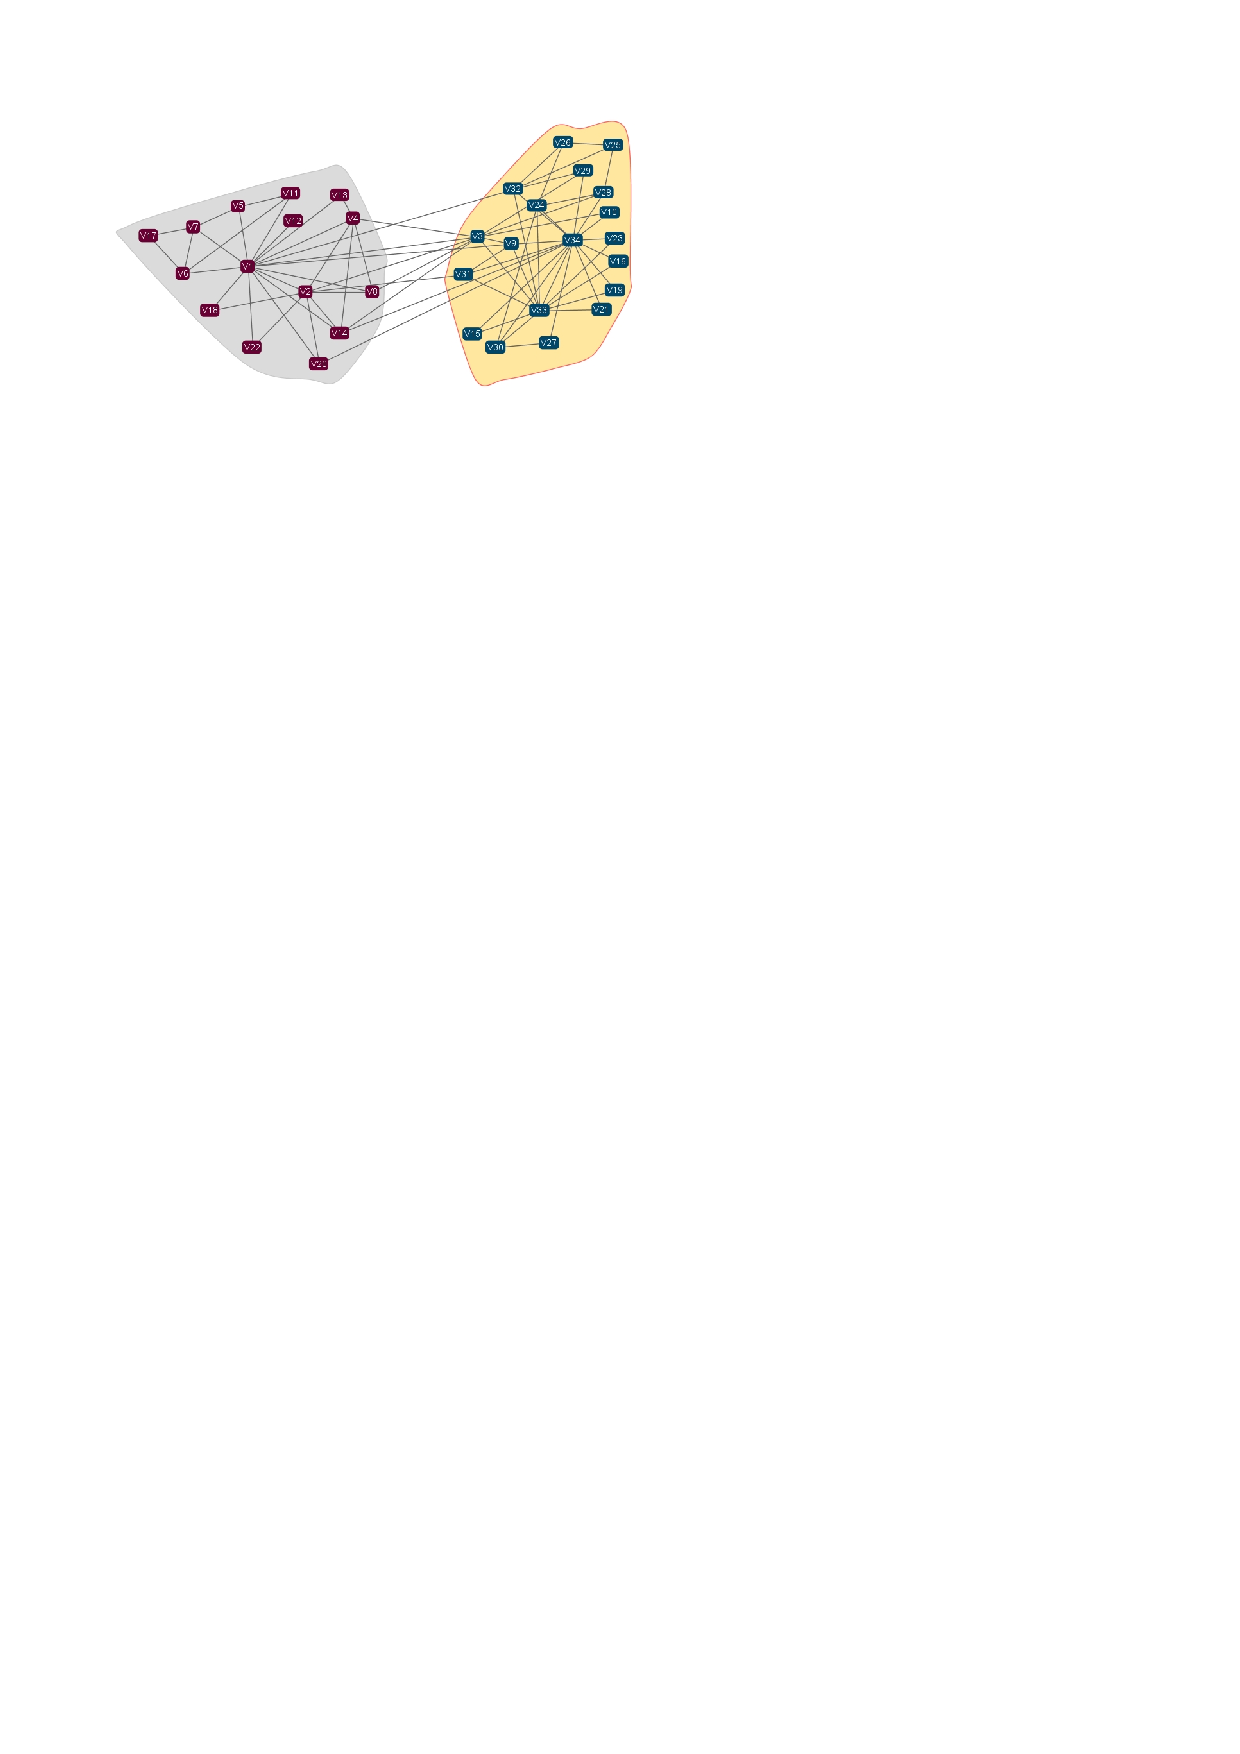
\includegraphics[height=4.5cm]{images/zacharyClub.pdf}
\end{center}
The algorithm detects two communities which exactly match with the result of Zachary’s study.
\end{frame}

%%%%%%%%%%%%%%%%%%%%%%
\begin{frame}{American college football}
\vskip 0.7cm
This network represents the schedule of Division I games for the 2000 season. 
\vskip 0.2cm
It consists of \textbf{115 vertices} and \textbf{616 edges} which are the representations of football teams and regular season games among them respectively. 
\vskip 0.2cm
115 teams are divided into \textbf{12 conferences} containing around 8 to 12 teams each. 
\vskip 0.2cm
Games are more frequent between members of the same conference than between members of different conferences. 
\vskip 0.2cm
Apparently, each conference can be considered as one community of the network.

\end{frame}

%%%%%%%%%%%%%%%%%%%%%%
\begin{frame}{American college football}
The algorithm shows an accuracy of 93.8\%.
\begin{center}
	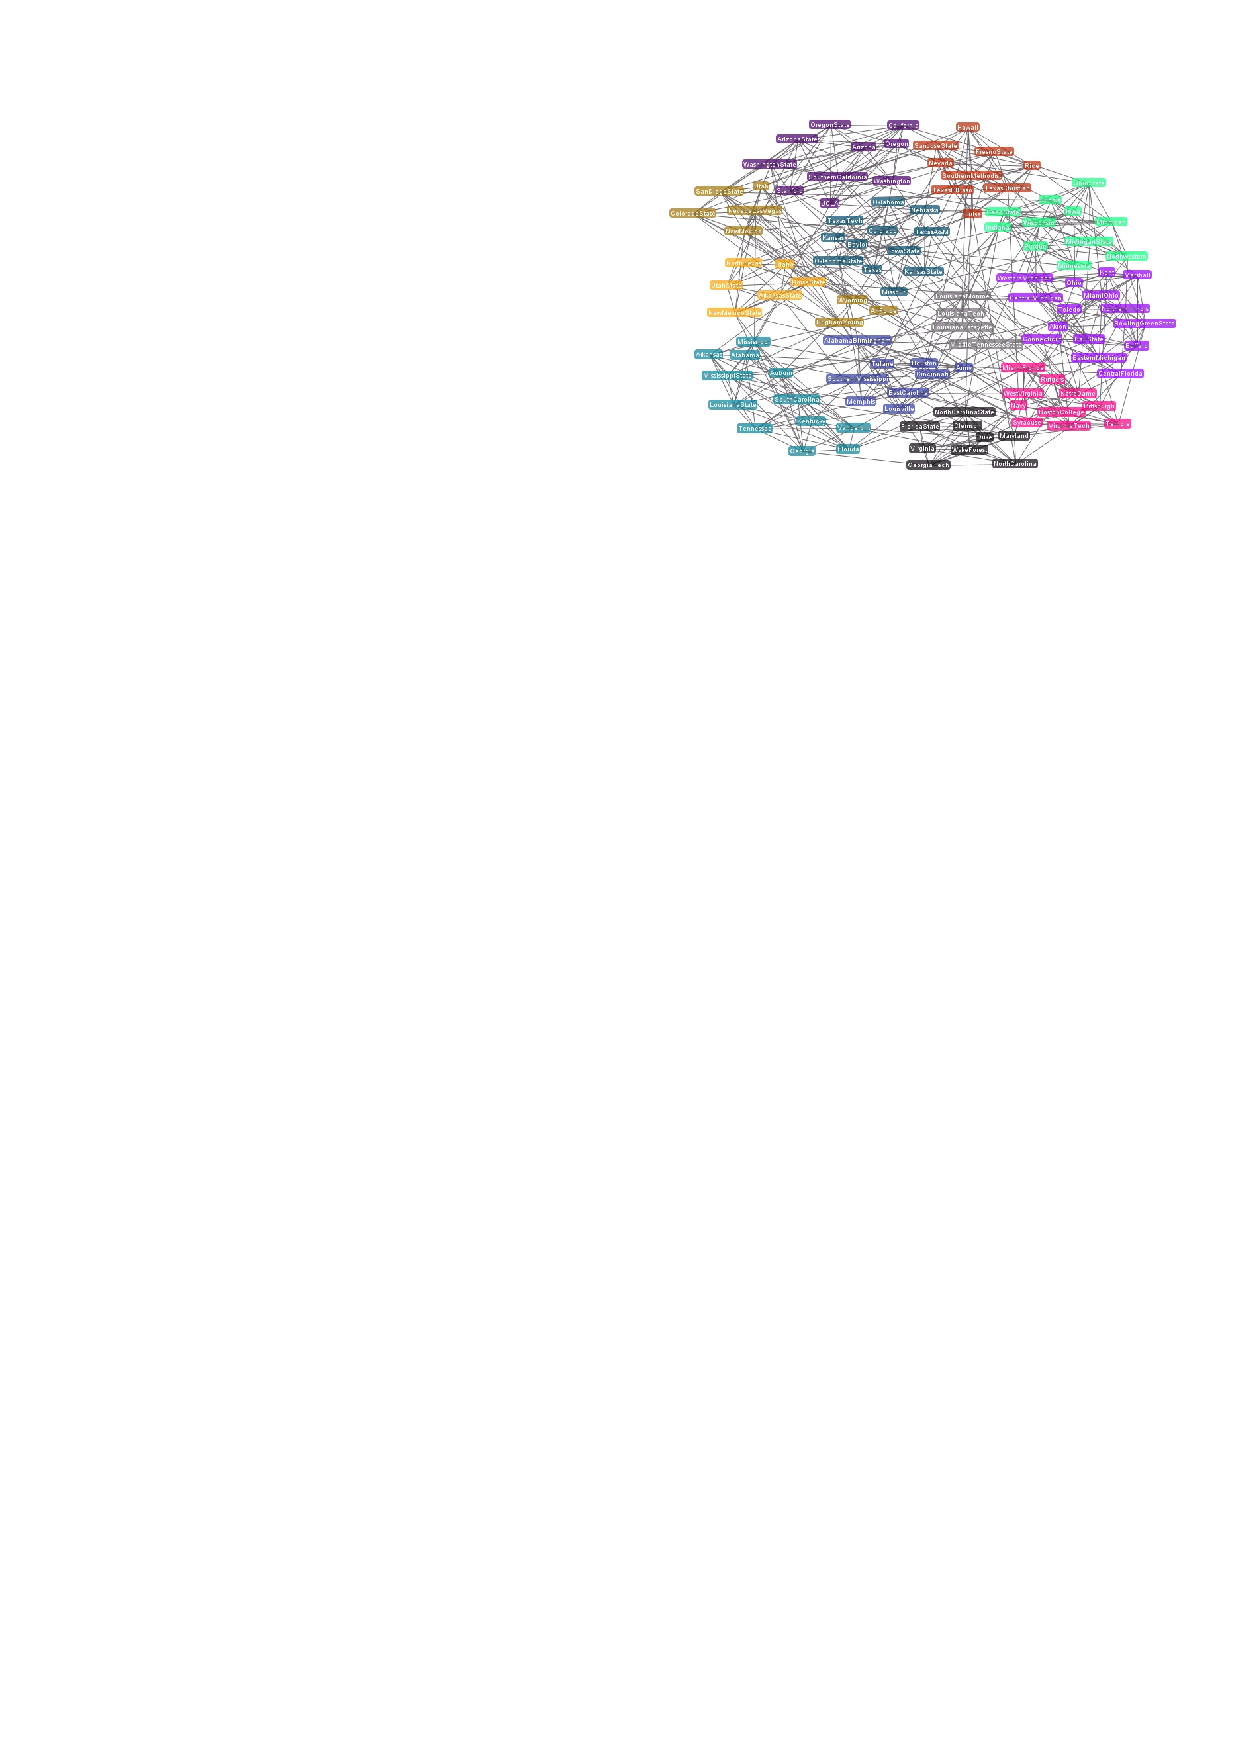
\includegraphics[height=7cm]{images/americanCollegeFootball.pdf}
\end{center}
\end{frame}

%%%%%%%%%%%%%%%%%%%%%%
\begin{frame}{Scientific collaboration}
\vskip 0.5cm
The data of the collaboration network is obtained according to the 1990 published papers from the year 1998 to 2005 indexed by SCI, EI and ISTP in Beijing University of Posts and Telecommunications(BUPT).
\vskip 0.6cm
Each \textbf{author corresponds to a vertex} of the network and \textbf{there is an edge between two vertices if the two correspondent authors have collaborated in a paper}.
\vskip 1cm
For each author it is created \textbf{a set of attributes} using the most relevant term in their papers.
\vskip 0.6cm
The \textbf{Periphery} area is an independent small component of the network, and the \textbf{Core} area corresponds to the giant component.
\end{frame}

%%%%%%%%%%%%%%%%%%%%%%
\begin{frame}{Scientific collaboration}
\begin{center}
	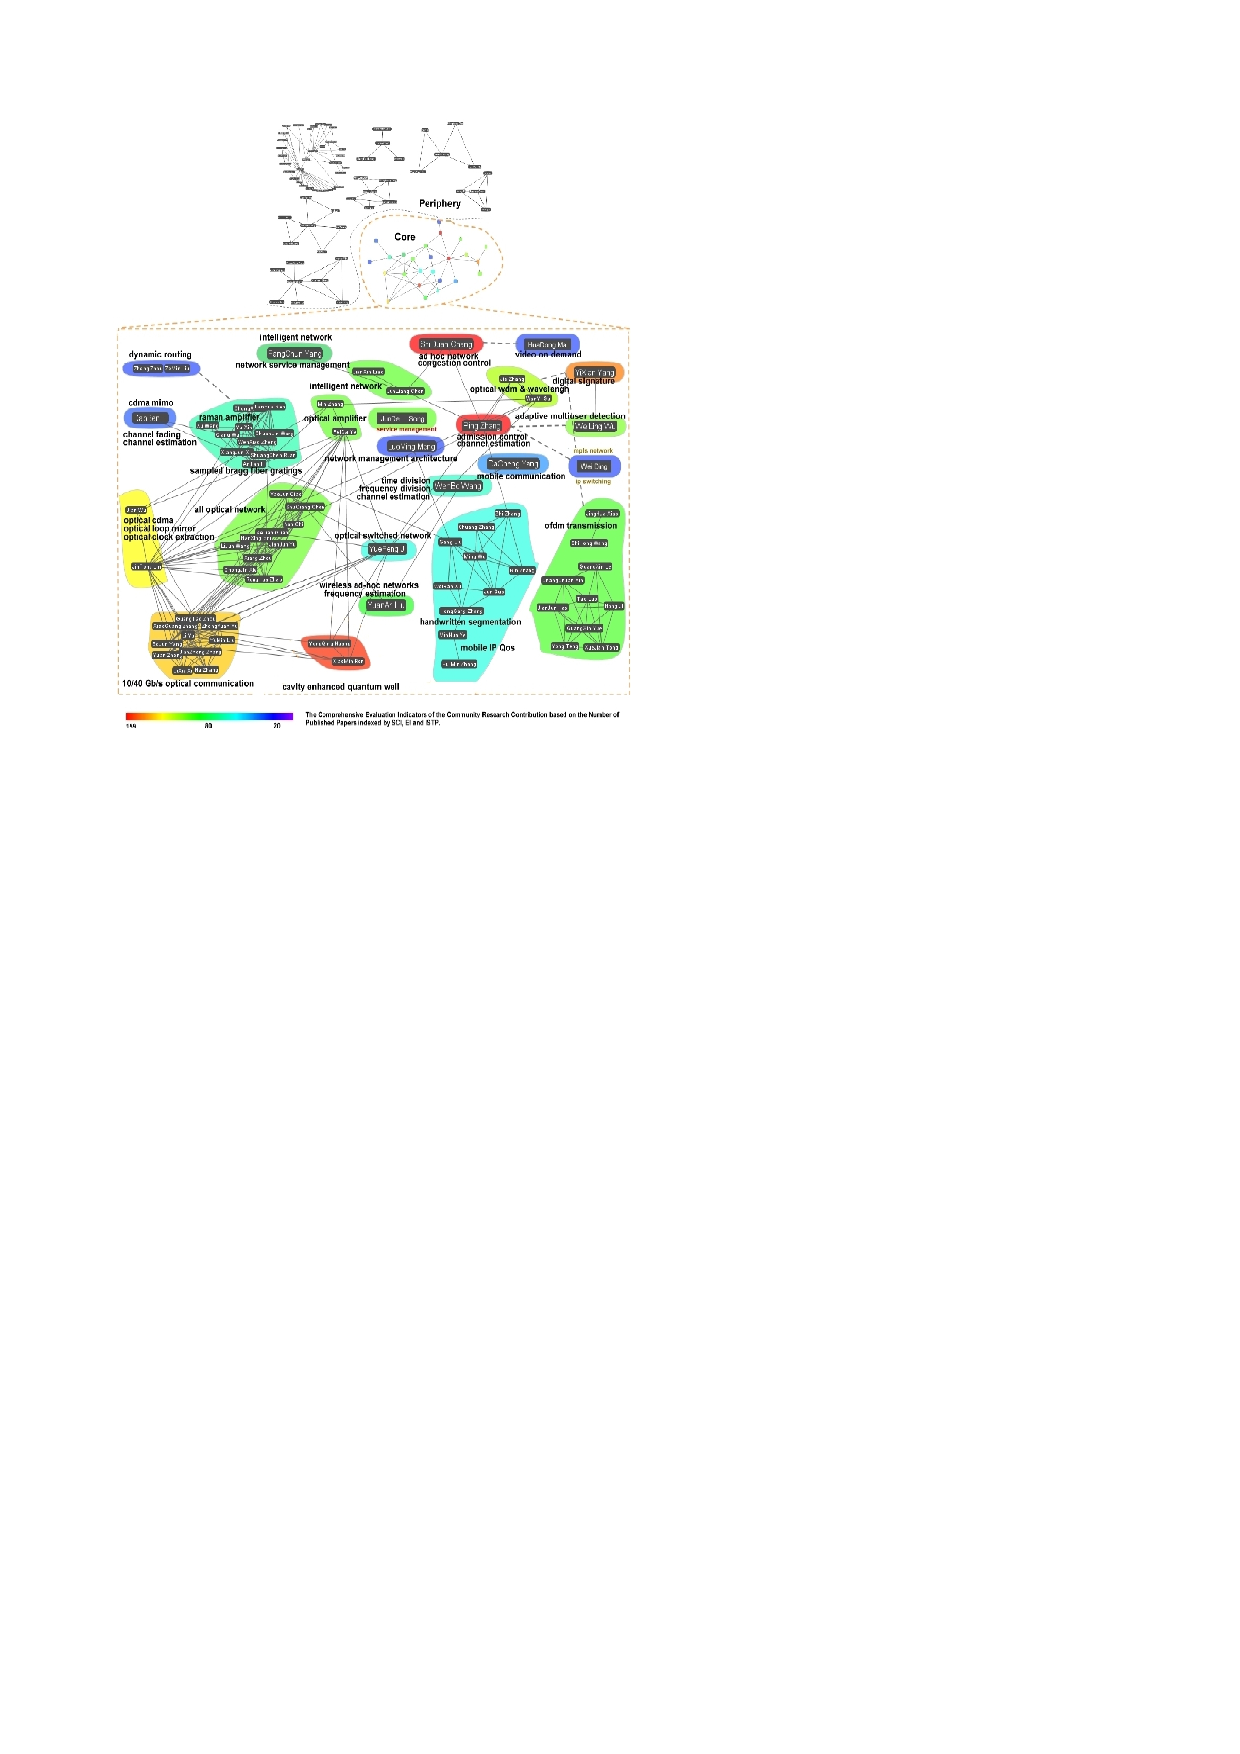
\includegraphics[height=8cm]{images/scientificCollaboration.pdf}
\end{center}
\end{frame}
